% Build with: latexmk -pdf -interaction=nonstopmode -halt-on-error concord.tex
% Self-contained article. All language fragments marked as proposed are specifications.
\documentclass[11pt,a4paper]{article}
\usepackage[T1]{fontenc}
\usepackage[utf8]{inputenc}
\usepackage{lmodern,microtype}
\usepackage[margin=24mm,headheight=15pt]{geometry}
\usepackage{amsmath,amssymb,amsthm,mathtools}
\usepackage{booktabs,longtable,tabularx,array}
\usepackage{xcolor,listings,tikz,enumitem,needspace,fancyhdr,titlesec}
\usepackage[most]{tcolorbox}
\usepackage{xurl,etoolbox}
\usepackage[colorlinks=true,linkcolor=blue!40!black,citecolor=blue!40!black,urlcolor=blue!40!black]{hyperref}
\usepackage{bookmark}
\usetikzlibrary{arrows.meta,positioning,fit}
\definecolor{ink}{HTML}{183447}
\definecolor{accent}{HTML}{1A7377}
\definecolor{pale}{HTML}{F1F6F7}
\definecolor{muted}{HTML}{536371}
\titleformat{\section}{\Large\sffamily\bfseries\color{ink}}{\thesection}{.6em}{}
\titleformat{\subsection}{\large\sffamily\bfseries\color{ink}}{\thesubsection}{.6em}{}
\titleformat{\subsubsection}{\normalsize\sffamily\bfseries}{\thesubsubsection}{.6em}{}
\setlength{\parindent}{0pt}
\setlength{\parskip}{.42em}
\setlength{\emergencystretch}{2.5em}
\setcounter{tocdepth}{1}
\pretocmd{\section}{\Needspace{9\baselineskip}}{}{}
\pretocmd{\subsection}{\Needspace{5\baselineskip}}{}{}
\setlist{nosep,leftmargin=1.5em}
\renewcommand{\arraystretch}{1.16}
\newcolumntype{Y}{>{\raggedright\arraybackslash}X}
\newcolumntype{P}[1]{>{\raggedright\arraybackslash}p{#1}}
\newcommand{\code}[1]{\nolinkurl{#1}}
\newcommand{\Concord}{\textsc{Concord}}
\newcommand{\N}{\mathbb N}
\newcommand{\Z}{\mathbb Z}
\newcommand{\Q}{\mathbb Q}
\newcommand{\R}{\mathbb R}
\newcommand{\C}{\mathbb C}
\newcommand{\E}{\mathcal E}
\newcommand{\den}[1]{\llbracket #1\rrbracket}
\newcommand{\coeff}[2]{[#1^{#2}]}
\newcommand{\Spec}{\operatorname{Spec}}
\newcommand{\Dom}{\operatorname{Dom}}
\newcommand{\checkc}{\operatorname{check}}
\newcommand{\var}{\operatorname{var}}
\newtheorem{proposition}{Proposition}[section]
\newtheorem{lemma}[proposition]{Lemma}
\theoremstyle{definition}
\newtheorem{definition}[proposition]{Definition}
\newtcolorbox{thesisbox}{colback=pale,colframe=accent!60,boxrule=.6pt,arc=1mm,breakable,left=9pt,right=9pt,top=7pt,bottom=7pt}
\lstset{basicstyle=\small\ttfamily,columns=fullflexible,keepspaces=true,
 breaklines=true,showstringspaces=false,frame=single,framerule=.3pt,
 rulecolor=\color{accent!40},backgroundcolor=\color{pale},framesep=5pt,
 aboveskip=.8em,belowskip=.6em,tabsize=2}
\pagestyle{fancy}
\fancyhf{}
\fancyhead[L]{\small\sffamily Concord: mathematical argument and verified computation}
\fancyhead[R]{\small\sffamily Second-round proposal}
\fancyfoot[C]{\thepage}
\hypersetup{pdftitle={Concord: A Query-Directed Proof Language with a Verified Symbolic Core},pdfauthor={OpenAI, prepared for Vladimir Reshetnikov},pdfsubject={Second-iteration proof-language proposal informed by Brainstorm, ProveIt, and Leant}}

\begin{document}
\begin{titlepage}
\color{ink}
{\sffamily\large PROOF-LANGUAGE DESIGN / SECOND ITERATION\par}
\vspace{22mm}
{\sffamily\bfseries\fontsize{34}{39}\selectfont Concord\par}
\vspace{7mm}
{\sffamily\bfseries\fontsize{24}{29}\selectfont A Query-Directed Proof Language\\with a Verified Symbolic Core\par}
\vspace{10mm}
{\Large Mathematical objects, human-scale arguments,\\and computations that carry their meaning\par}
\vspace{12mm}
\begin{thesisbox}
\textbf{The proposal.} Make a mathematical query---not a tactic call and not an unqualified CAS expression---the boundary between an author's idea and automatic computation. Every answer records what it establishes: an equality, a coefficient, a local derivative, a complete solution set, or a certified enclosure. The author controls the mathematical choices; theorem-backed algorithms and certificate checkers reconstruct the consequences.
\end{thesisbox}
\vfill
\rule{\textwidth}{.7pt}
Prepared for Vladimir Reshetnikov\par
OpenAI\par
5 September 2026, Pacific time\par
\vspace{5mm}
{\small This is an original design proposal grounded in a close reading of both Brainstorm synthesis reports and selected committed ProveIt and Leant sources. It contains mathematical derivations, proposed syntax, interface specifications, and an experimental plan. It does not claim an implemented language, a formally verified compiler, or measured usability gains.}
\end{titlepage}

\begin{abstract}
The first brainstorm round reached a useful consensus: retain Lean, expose mathematical steps, reconstruct scoped obligations, fix meaning independently of proof search, and preserve accepted evidence. A second round should not merely give this architecture another vocabulary. This article proposes a particular extension: a query-directed language whose symbolic-computation layer is based on theorem-backed algorithms, verified checkers, and explicitly typed relations between mathematical objects and computational representations.

The central design unit is a \emph{contracted query}. Its output is not merely a value. It includes the specification that the value satisfies, its domain and branch commitments, its precision or locality, and any still-open obligations. Proof development and computer algebra consequently use one interface. An author can ask for a coefficient without computing an entire series, a root without silently choosing a branch, or a derivative without promoting equality at a point to equality in a neighborhood.

The contribution beyond the earlier reports is a concrete account of computational meaning and representation composition: demand-indexed observations; definition packages with verified implementations; conditional, case-split, exact, and approximate answers; and a strict distinction between algorithm correctness and evidence for a particular execution. Worked examples preserve the additive-group generality of binomial inversion, the local hypotheses of autonomous differentiation, and the arbitrary rational-algebra setting of Abel generating functions. Additional examples cover radical denesting, complete root sets, exact algebraic numbers, and certificate-based polynomial reasoning. The proposal also sharpens the Leant boundary: a fragment-completeness flag is useful metadata, but neither that flag nor search exhaustion is an object-level proof of negation.

A small shared implementation with ordinary Lean and mathematical frontends is recommended. Its success should be measured by mathematical choice, repair cost, explanatory accuracy, and total development effort, not by source-line compression alone.
\end{abstract}
\clearpage
\tableofcontents
\clearpage

\section{The second-round thesis}\label{sec:thesis}

\subsection{Keep the consensus; change the center of gravity}
The two synthesis reports agree on most of the important foundations. A readable proof should display its mathematical assertions and choices; omitted reasoning must remain scoped and checkable; search must not choose a more convenient theorem than the one the author stated; and the accepted evidence should survive the disappearance of the search that found it. They also agree that the comparison must give ordinary Lean the same auxiliary lemmas and automation as the proposed frontend~\cite{synA,synB}.

I accept that common core. I do not propose a new foundational logic, a replacement for Lean's kernel, or unrestricted natural language as an authoritative input format. My departure is to treat \emph{mathematical computation as a first-class part of the language}, rather than merely one of the tactics that can close a proof obligation.

A mathematician routinely alternates between asserting and calculating:
\begin{quote}
Choose this representation. Compute the coefficient that matters. Factor the resulting polynomial. Select the positive root. Differentiate the identity where it holds. The remaining conditions follow from the hypotheses.
\end{quote}
A conventional CAS emphasizes the resulting expression. A proof assistant emphasizes a proposition and its evidence. \Concord{} would emphasize a \emph{query and its mathematical contract}: which object is being observed, which result is sought, and exactly what relationship must be established.

\begin{thesisbox}
\textbf{Design principle.} Every automatic operation must answer a question that is already mathematically meaningful. A returned expression is accepted only together with evidence answering that question. When the answer is conditional, partial, approximate, or branch-dependent, those qualifications belong to the answer's type and presentation.
\end{thesisbox}

This is not a claim that proof assistants and computer algebra have never been combined. Verified algebraic-number implementations, certificate-based real-algebra procedures, and verified numerical-error checkers already demonstrate important pieces of that combination~\cite{algnums,univariate,flover}. The proposed contribution is their integration into a concise language of mathematical arguments, with a particularly explicit account of observations, definitions, and compositional computational contracts.

\subsection{What is actually new in this iteration?}
The following table separates inherited architecture from the proposed extension. ``New'' here means new emphasis or additional specification relative to the two synthesis reports, not historical priority.

\begin{tabularx}{\textwidth}{@{}P{.28\textwidth}YY@{}}
\toprule
Concern & Inherited commitment & Additional proposal here\\
\midrule
Mathematical steps & Typed claims and theorem-backed methods. & Queries that produce specified mathematical data, not only proofs.\\
Representation & Certified views with recorded routes. & Observation-indexed transport laws and a concrete composition discipline.\\
Definitions & Compare alternative representations. & Definition packages coupling specification, implementation, and query interface.\\
Computation & Proof-producing automation behind obligations. & Explicit algorithm/checker/execution boundaries and heterogeneous answer relations.\\
Precision & Do not confuse formal and analytic objects. & Demand-indexed finite jets, enclosures, and locality with checked weakening rules.\\
Witnesses & Retain data choices and their specifications. & Automatic replacement only under an appropriate uniqueness or observational transport theorem.\\
Search outcomes & Exhaustion is not refutation. & Separate logical negation, countermodels, and metatheoretic nonderivability.\\
\bottomrule
\end{tabularx}

\subsection{What the language must not promise}
The system is not expected to compute arbitrary real numbers exactly, decide equality of arbitrary functions, infer every useful induction invariant, or find an elementary expression whenever one exists. A query may remain open or be unsupported by the installed computational fragment. That is a limitation of a particular capability, not a reason to misstate the mathematics.

Nor should concision mean that substantial assumptions disappear. The domain of a logarithm identity, domination in a limit interchange, the invertibility of a coefficient, and the branch of an algebraic root can be central parts of the argument. The system should suppress repetitive \emph{proofs of already justified conditions}, not suppress the conditions' mathematical role.

\section{Reading the evidence carefully}\label{sec:evidence}

\subsection{Sources and revision boundaries}
Both requested synthesis reports were read closely, including their mutual corrections, questions for the next round, and source notes. Their summaries are sufficient for the first-round comparison here; I do not claim to have independently reread all nine underlying proposals. Direct code inspection concentrates on three ProveIt modules and the committed Leant verification, fragment-translation, and suggestion paths~\cite{synA,synB,pbin,pode,pabel,lverify,lfragment,lmain}.

\begin{tabularx}{\textwidth}{@{}lP{.27\textwidth}Y@{}}
\toprule
Repository & Inspected revision & Qualification\\
\midrule
Brainstorm & \code{494be9d5ab41} & Both synthesis sources, including the latest second-round questions.\\
ProveIt & \code{24ce8bd743ea} & Public main revision returned during this review; three complete Lean modules.\\
Leant & \code{3a40904be8a4} & Committed sources; not the unpublished working tree described in the syntheses.\\
\bottomrule
\end{tabularx}

The complete commit identifiers and paths are in the references and source register. The syntheses also inspected a ProveIt checkout at \code{7c4e3f10} and modified Leant working-tree files. Those are not silently substituted for the public revisions inspected here. In particular, their discussion of an uncommitted behavioral \code{where} extension is treated as an attributed report, not as a feature newly executed or independently validated for this article~\cite{synA,synB}.

No ProveIt or Leant build was run. Source inspection can establish what an inspected code path says; it does not establish its runtime behavior in every environment. The accompanying exact-arithmetic checks concern the article's small mathematical examples only, not those repositories.

\subsection{Three examples, three different sources of friction}
\textbf{Binomial inversion.} The long part of \code{BinomialInversion.lean} exposes an index change, natural-number bounds, a binomial product identity, scalar casts, and polynomial rearrangement. Its final transforms are already factored through a reusable lower-triangular-kernel framework. Importantly, the principal transform theorem works in any additive commutative group, using integer scalar multiplication. A replacement that only works over a field would be a regression in the theorem, however attractive its surface text~\cite{pbin}.

\textbf{Autonomous differentiation.} The proof of \code{AutonomousODE.iteratedDeriv_eq_comp} is already compact and mathematically organized. Its representational work is the transfer from an identity throughout an open set to eventual equality near the current point, followed by the chain rule. The assumptions on the auxiliary functions hold only at values reached by the solution. A new frontend should preserve that locality, not replace it with global smoothness because global assumptions are easier for automation~\cite{pode}.

\textbf{Abel generating functions.} \code{AbelPolynomialSeries.lean} separates a canonical series construction from a coefficient theorem for \emph{any} series satisfying the defining equation. The proof uses formal substitution, Lagrange inversion, exponential identities, and rational-scalar transport into an arbitrary commutative \(\Q\)-algebra. This is an especially good hybrid test: the symbolic calculation is highly regular, but its algebraic and formal-series meaning must remain intact~\cite{pabel}.

These examples do not support the blanket claim that Lean is a bad language or that all detailed proofs should be rewritten. They suggest that a computational interface can expose a reusable mathematical operation while absorbing predictable representation work. Some existing one-line corollaries should remain one-line Lean corollaries.

\subsection{What the two syntheses settle---and what they do not}
The first synthesis's strongest contribution is the separation of target fidelity, checked proof evidence, document coverage, and method conformance. The second's strongest additional implementation proposal is that a method's logical contract should normally be an ordinary theorem with role annotations, rather than a separate contract calculus duplicating its type. Both positions are adopted below~\cite{synA,synB}.

The reported corpus audit is useful for choosing test families. Its 90,637 classified tactic-like entries and approximately 32\% in selected bookkeeping families are lexical observations, not measured removable work. They do not justify a promised compression percentage. Likewise, finding existing tactics for a family does not show that their inputs, failures, or explanations are already natural to a mathematician~\cite{synB,synA}.

One issue needs further sharpening. The second synthesis describes Leant's safety metadata as an operational form of adequacy. Such metadata is useful, but it is not itself a proof that a translation preserves an original mathematical problem, and nonderivability in a proof-search calculus need not be a proof of the original proposition's negation. Section~\ref{sec:negative} makes the distinction concrete.

\section{The author's experience}\label{sec:surface}

\subsection{A small surface over a richer semantic object}
The initial frontend should reuse Lean expressions and declarations, adding a mathematical block and a query interface. The more mathematical notation below is \emph{proposed syntax}, not executable Lean. Its purpose is to specify interactions and meanings, not to claim an implemented parser.

\par\noindent\begin{minipage}{\linewidth}
\begin{lstlisting}
context A : commutative Q-algebra
  let a, x : A
  let T : formal_series A
  assume defining : T = z * exp(-a * T)

  theorem abel_coefficient(n : Nat):
    coefficient(z^(n+1), exp(x*T))
      = scalar(1/(n+1)!) * x * (x - (n+1)*a)^n
  proof
    use Lagrange_inversion on defining
      with outer u |-> exp(x*u)
    compute the resulting coefficient
      using formal_exponential_rules
    normalize rational scalars in A
  end
end
\end{lstlisting}
\end{minipage}\par

The apparent simplicity relies on explicit interfaces. \code{formal_series A} is not an analytic function. \code{scalar} means the chosen map from \(\Q\) to \(A\). The formal variable and all interval conventions have fixed meanings in the context. The Lagrange step creates its actual premises from a theorem. The two computational steps return evidence for exact identities in the selected algebra.

An author should not have to inspect a raw proof term to understand these choices. A compact expanded header might say:
\begin{quote}
Arbitrary commutative rational algebra; formal series, not analytic functions; arbitrary solution of the displayed equation; coefficient index is \(n+1\); scalar reciprocals are computed in \(\Q\) and mapped into the algebra.
\end{quote}
This display discloses resolved semantics. It does not certify that they match the author's intention; that remains a review task.

\subsection{Queries are not all assertions}
A proof step can start with a claim whose evidence is missing, or with a computation whose value is missing. These should be different operations:
\par\noindent\begin{minipage}{\linewidth}
\begin{lstlisting}
claim orthogonality : K * L = identity
  by finite_kernel_composition

compute p := coefficient(z^8, exp(x*T))
  as polynomial in [a, x] over Q

find r : Real satisfying r > 0 and r*r = a
  using positive_root

explore factorization of p
\end{lstlisting}
\end{minipage}\par

\code{claim} fixes a proposition. \code{compute} fixes an output specification and asks for its value. \code{find} intentionally leaves a data choice open subject to a specification. \code{explore} may show conjectures, heuristics, or unchecked outputs, but none may become an accepted theorem premise simply because it appears in the notebook.

A deterministic normal form can usually be accepted automatically when its denotation is certified. Selecting an arbitrary root cannot be treated the same way. Multiple candidates may be shown during exploration; publication retains the chosen object and its complete specification, not just its type.

\subsection{A useful failure is a mathematical explanation}
Suppose an author writes:
\par\noindent\begin{minipage}{\linewidth}
\begin{lstlisting}
compute sqrt(x*x) = x
\end{lstlisting}
\end{minipage}\par
For real \(x\), the universal assertion is false. The system should distinguish a failed selected normalization from a refutation. A useful response is:
\begin{quote}
The principal-square-root rule gives \(\sqrt{x^2}=|x|\). Rewriting the result to \(x\) needs \(0\leq x\). That condition is not available. The unconditional assertion fails at \(x=-1\).
\end{quote}
The identity with absolute value, the residual obligation, and the counterexample require separate evidence. If the system has only failed to establish \(0\le x\), it may report that missing condition, but must not invent the counterexample or call the ambient theorem false.

The three valid next actions are to keep \(|x|\), prove nonnegativity from existing assumptions, or explicitly split into sign cases. Adding \(x\ge0\) to the theorem is a statement edit, not automatic proof progress.

\subsection{Visible decisions; expandable consequences}
Default presentation should expose the index map, induction invariant, chosen branch, computational domain, and significant regularity premises. It can collapse a proof that a bounded index is nonnegative, a routine cast lemma, or exact rational arithmetic. This is not a permanent classification of propositions into important and unimportant ones. In a theorem about natural subtraction, the bound licensing a cast may be the whole mathematical point.

Every source claim remains linked to its evidence even if unused later. A true conclusion does not excuse a false intermediate assertion. Free prose can explain the document, but only expressions linked to formal assertion nodes receive a checked status. The interface should never paint an entire paragraph as verified merely because one formula in it was checked.

\section{A small semantic core for claims and computations}\label{sec:core}

\subsection{The mathematical contract of a query}
A query \(q\) has an input type \(I_q\), an output type \(O_q(i)\), and a specification
\[
  \Spec_q(i,y):\mathrm{Prop},\qquad i:I_q,\quad y:O_q(i).
\]
The input includes the resolved mathematical environment: coefficient structure, branch policy where applicable, conventions, and the requested observation. An accepted answer consists of a value \(y\) and a proof of \(\Spec_q(i,y)\). In schematic dependent-type notation:
\par\noindent\begin{minipage}{\linewidth}
\begin{lstlisting}
structure CheckedAnswer (q : Query) (i : q.Input) where
  value    : q.Output i
  evidence : q.Spec i value
\end{lstlisting}
\end{minipage}\par
This is an interface sketch. It is not enough to manufacture a host-language record called \code{CheckedAnswer}; the evidence must be checked at the exact specification in the recorded Lean environment.

The specification need not be an equality. A factorization query can request a product identity; an irreducible-factorization query additionally requests irreducibility. A root query can request one root; a complete-solving query additionally requests that every solution occurs in the returned representation. A numerical query can request a rational enclosure rather than an exact real value. Distinct specifications prevent a successful weaker computation from being presented as a stronger answer.

\begin{tabularx}{\textwidth}{@{}P{.22\textwidth}P{.26\textwidth}Y@{}}
\toprule
Query & Output & Required mathematical evidence\\
\midrule
Normalize & Expression or polynomial & Equal denotation in the declared algebra.\\
Factor & Factors and multiplicities & Product identity; completeness or irreducibility only if separately requested.\\
Solve completely & Finite roots or a case description & Both solution soundness and solution coverage in the declared domain.\\
Differentiate & A derivative expression & A local derivative relation with its domain, not merely a symbolic string.\\
Extract coefficient & A coefficient expression & Equality to the specified coefficient of the original formal series.\\
Enclose & Rational bounds & Containment of the original mathematical value.\\
Choose witness & Data object & The full requested property, with its dependence on earlier variables.\\
\bottomrule
\end{tabularx}

\subsection{Conditional answers and residual obligations}
A useful computation often discovers its own premises. Cancellation may require a nonzero denominator; a symbolic inverse may require a unit; a substitution may require a vanishing constant term. These conditions must not be silently assumed.

Represent a conditional answer by a telescope \(\Delta\) of still-open obligations, a result \(y\) defined in \(\Gamma,\Delta\), and evidence
\[
  \E;\Gamma,\Delta\vdash y:O_q(i),
  \qquad
  \E;\Gamma,\Delta\vdash c:\Spec_q(i,y).
\]
The telescope is ordered: later entries can depend on earlier entries. Its members can include proof obligations and explicitly marked data choices. Closing over it produces a well-typed conditional artifact, not a proof of the unconditional query. An unguarded consumer cannot use \(y\) until the required arguments are supplied.

This gives two legitimate user experiences. A step may pause and display its remaining conditions, or a subsequent step may inherit exactly the same pending telescope. Neither behavior introduces an axiom. A publication claiming the unconditional result must discharge the obligations. Publishing a conditional theorem instead is possible, but must display the conditional statement as such.

This matters even if the resulting expression happens not to contain the guard syntactically. The identity \(x/x=1\) needs \(x\ne0\) under ordinary field division conventions; the constant expression \(1\) does not reveal that dependency. Evidence provenance, not free variables of the output expression alone, determines the obligations.

\subsection{Theorems, algorithms, and structural plans}
The logical contract of a method should usually be an ordinary Lean theorem. A reindexing theorem's hypotheses generate membership, injectivity, coverage, and summand obligations. A local differentiation theorem generates neighborhood equality and derivative premises. Role annotations specify which inputs the author selects and which premises a routine profile may attempt~\cite{synA,synB}.

Roles should refer to stable slots in a project-owned wrapper, with a checked mapping to the underlying theorem's telescope. Merely changing positional flags to binder names does not solve renaming. A wrapper declaration gives the project a compatibility boundary: if Mathlib changes its theorem, one adapter is repaired, rather than silently retargeting roles throughout the document. Policy versions remain separate from theorem versions.

There are three implementation forms, not one universal method language:
\begin{enumerate}
\item \textbf{Theorem application:} instantiate an ordinary theorem and expose its premises.
\item \textbf{Certified computation:} run a specified algorithm or validate a proposed answer with a proved checker.
\item \textbf{Structural elaboration:} construct an induction, case split, or local context using the host's eliminators and scoped terms.
\end{enumerate}
All three produce the same kind of checked query or claim node. They need not share their internal search algorithm. A structural plan is not made safe merely by disguising it as one more arbitrary string-valued method name.

\subsection{The status is a vector, not a green light}
A node has several independently meaningful statuses: its statement may be resolved or ambiguous; its mathematical evidence may be complete or conditional; its computation may be exact or enclosing; its method may conform to the advertised plan or merely establish the checkpoint; its replay may have been independently checked or only accepted in a live session.

A user-facing summary can remain compact. For example:
\begin{quote}
Exact coefficient established; two scalar identities discharged; formal-series domain; method conforms to Lagrange inversion; retained evidence replayed.
\end{quote}
The underlying record must retain the distinctions. In particular, ``fewer goals'', ``this goal closed'', ``the whole declaration complete'', and ``the exact proposed edit independently replayed'' are different facts.

\section{What makes the symbolic core formally verified?}\label{sec:cas}

\subsection{Three layers that must not be conflated}
A claim that a CAS uses a verified algorithm can mean several things. \Concord{} should distinguish the mathematical algorithm theorem, the implementation/refinement theorem, and the evidence for the concrete run that produced the returned answer.

For a total pure algorithm \(f\), the ideal specification is
\[
  \forall i,\ \Spec(i,f(i)).
\]
If an external process returns \(y\), that theorem alone does not prove \(\Spec(i,y)\). The checking path still needs evidence that \(y=f(i)\), or a separate certificate establishing the specification directly. Running a formally specified algorithm through an unverified compiler does not, by itself, authenticate arbitrary output bytes.

\begin{center}
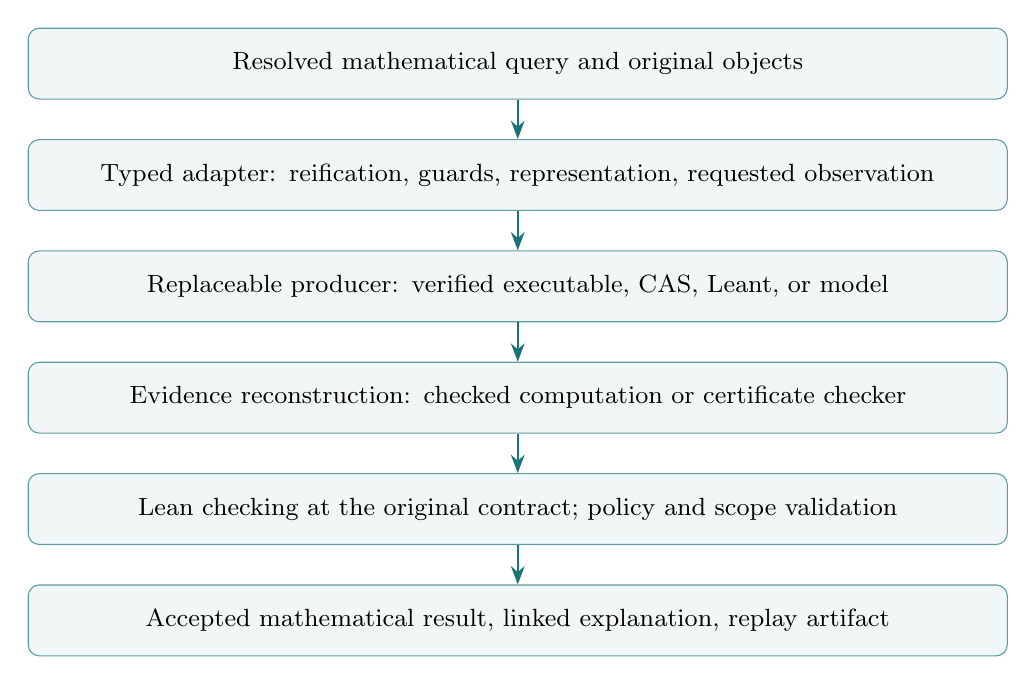
\begin{tikzpicture}[node distance=5mm,>=Stealth,
 box/.style={draw=accent!70,rounded corners,fill=pale,align=center,
 text width=12.2cm,minimum height=9mm,font=\small}]
\node[box] (a) {Resolved mathematical query and original objects};
\node[box,below=of a] (b) {Typed adapter: reification, guards, representation, requested observation};
\node[box,below=of b] (c) {Replaceable producer: verified executable, CAS, Leant, or model};
\node[box,below=of c] (d) {Evidence reconstruction: checked computation or certificate checker};
\node[box,below=of d] (e) {Lean checking at the original contract; policy and scope validation};
\node[box,below=of e] (f) {Accepted mathematical result, linked explanation, replay artifact};
\foreach \x/\y in {a/b,b/c,c/d,d/e,e/f}\draw[->,thick,accent] (\x)--(\y);
\end{tikzpicture}
\end{center}
The producer's implementation can change without changing the query's mathematical meaning. The input and claimed output are both included in what the checker validates; a certificate is not checked against a conveniently reconstructed substitute problem.

\subsection{Execution route A: checked evaluation of a proved algorithm}
For small or moderate exact computations, the system can define a normalizer in Lean, prove its denotational correctness, and evaluate it through a checking route accepted by the project's trust policy. For example:
\[
 \operatorname{eval}(\operatorname{nf}(e),\rho)
   =\operatorname{eval}(e,\rho)
\]
for a polynomial syntax \(e\) and an interpretation \(\rho\). Equality of two computed normal forms then yields an identity in every permitted interpretation.

The logical assumptions should be no stronger than the theorem needs. Polynomial normalization in a commutative ring is different from cancellation in a field. Normalizing an identity over \(\Q[a,x]\) and transporting it along an evaluation homomorphism does not require decidable equality of arbitrary real numbers or arbitrary coefficients in the target algebra.

The price is checking cost. Kernel reduction of a large computation may be much more expensive than its native execution. The language must budget checking as well as discovery. Calling a computation ``routine'' does not make its proof cheap.

\subsection{Execution route B: verified checker, replaceable producer}
For expensive search, use a certificate relation
\[
 \checkc(i,y,c)=\mathrm{true}
 \quad\Longrightarrow\quad \Spec(i,y),
\]
with a correctness theorem proved in Lean. A fast producer proposes \(y,c\); a permitted checking route establishes the Boolean equality and applies the theorem. The producer may itself be a verified implementation, but it need not be trusted for the result's logical authority.

A polynomial consequence is a simple example. Given hypotheses \(p_1=\cdots=p_m=0\), a producer proposes polynomials \(q_i\) such that
\[
       p=\sum_{i=1}^{m}q_i p_i.
\]
Checking this identity establishes \(p=0\) in any commutative ring. Discovering the \(q_i\) can be difficult; verifying the displayed algebraic identity is a smaller, deterministic problem. If the certificate instead establishes \(p^k=\sum_iq_ip_i\), concluding \(p=0\) needs an appropriate hypothesis excluding nonzero nilpotents. It is invalid in an arbitrary commutative ring. The certificate format must distinguish those conclusions.

The same architectural separation appears in the Isabelle/HOL work on univariate real polynomial problems, where external algebraic computation produces certificates checked inside the logic~\cite{univariate}. That precedent motivates the boundary; it is not evidence that the corresponding Lean implementation already exists.

\subsection{Execution route C: proof-producing transformations}
Some operations are best implemented by composing existing lemmas, yielding an ordinary proof term rather than evaluating one monolithic verified program. Symbolic differentiation is a natural example: expression traversal proposes a derivative, while chain, product, and quotient rules assemble local derivative proofs. A function outside the recognized syntax remains an opaque mathematical object with an explicit derivative premise.

This route is already close to ordinary proof-producing automation. Its addition here is an object-producing contract, the preservation of locality and branch information, and a durable link from the answer to the original query. It is a bridge toward a verified CAS, not a pretense that every tactic has been formally proved correct as a program.

\subsection{Trust profiles must disclose native computation}
The default publication profile should accept ordinary checked evidence under an explicit axiom allowlist, excluding computation-specific admissions. A separate profile may permit a larger trusted execution base, but it must label that choice. Current Lean documentation states that native evaluation introduces dedicated axioms for computations in versions from 4.29 onward; looking only for an older single constant is therefore inadequate~\cite{leanvalidate}.

The project should pin the exact Lean and library versions, inventory the actual transitive axioms, and check every declaration used by an answer. A proof can be valid relative to its assumptions while failing the selected publication policy. Policy rejection must not be confused with a mathematical refutation.

\subsection{The first computational scope should be deliberately narrow}
An initial symbolic core should support exact integer and rational arithmetic, polynomial identities, guarded rational expressions, finite index transformations, and a formal-series coefficient interface. Local differentiation can use theorem-producing syntax traversal. Real algebraic numbers and certified enclosures can follow behind the same contracts.

The implementation should not initially promise complete integration, general radical denesting, arbitrary transcendental simplification, or automated asymptotic analysis. Such capabilities can be added one theorem family or checker at a time. An external CAS may propose a candidate even when no complete search algorithm is available; the candidate can still be valuable if its exact mathematical specification is checked.

There is a practical reason to avoid a permanent dependence on a particular service. The current Mathlib documentation says that \code{polyrith} is no longer supported because its external Sage service closed; it points to \code{grobner} for polynomial reasoning, with different suggestion behavior~\cite{polyrith}. This does not alter the pinned source observations in the earlier reports. It does make service-independent certificates and offline replay a concrete requirement rather than merely an architectural preference.

\section{Definitions and representations as mathematical interfaces}\label{sec:views}

\subsection{A definition package is not a bag of coercions}
A definition package contains a mathematical specification, one or more concrete representations, proved observation laws, explicit domain conventions, and a versioned simplification policy. The central mathematical object need not be executable. Its computational representation must implement the observations used by a query.

For a formal series, the semantic object might be an element of \(A[[z]]\). A computational representation might be a finite array of coefficients, together with a theorem relating the array to a specified initial segment of the series. For a real algebraic number, a representation might be a polynomial and isolating interval, together with existence and uniqueness evidence. For a bounded function, a bundled object can carry its bound once rather than reconstructing that condition after every use.

These are library assets, available equally in ordinary Lean. The language contributes their explicit selection, demand propagation, obligation display, and stable use in a document. It should not claim library abstraction as a uniquely linguistic achievement.

\subsection{Observation-indexed views}
Let \(A\) be a mathematical type, \(B\) a representation type, and \(V(a,b)\) a relation saying that \(b\) represents \(a\). A query observes an \(a\) through a specified function or relation. The representation is useful only if a proved transport law connects the relevant observations.

For exact observations \(o:A\to C\) and \(\widehat o:B\to C\), the law may be
\[
       V(a,b)\ \Longrightarrow\ o(a)=\widehat o(b).
\]
For a numerical enclosure it may instead be
\[
       V(a,b)\ \Longrightarrow\ o(a)\in\widehat o(b).
\]
A single global equality between mathematical object and representation is neither necessary nor usually well typed. A list of initial coefficients is not equal to a formal series, but it can answer every coefficient query in a certified range.

Likewise, preservation and reflection differ. A homomorphism preserves equations; it need not reflect them. For example, the map \(\Z\to\Z/2\Z\) sends \(0\) and \(2\) to the same value. A proof of equality after that map is not a proof of equality before it. Every backward proof step must name the actual reflection theorem it uses.

\subsection{Composing guarded views}
Suppose a first view relates \(a:A\) to \(b:B\), under a guard \(H(a,b)\), and a second relates \(b\) to \(c:C\), under a guard \(K(b,c)\). A composed representation is justified by the dependent data
\[
  \exists b,\ H(a,b)\land V(a,b)\land K(b,c)\land W(b,c).
\]
When the particular intermediate object is retained, the existential is represented by that object and its evidence. The order matters: the second guard is evaluated at the actual output of the first step, not at an unrelated expression with the same printed name.

\begin{proposition}[Composition at a demanded observation]\label{prop:views}
Suppose \(V(a,b)\) implies \(o_A(a)=o_B(b)\), and \(W(b,c)\) implies \(o_B(b)=o_C(c)\). Under the guards required by the two view instances, their retained certificates yield \(o_A(a)=o_C(c)\).
\end{proposition}
\begin{proof}
Instantiate both transport theorems at the retained intermediate object \(b\), then compose the two equalities. If the second representation or its type depends on the first guard, instantiate that dependency before applying its transport theorem. One cannot replace this ordered instantiation by collecting untyped guard strings in a set.
\end{proof}

The equality presentation is the simplest case. Containment, implication, local equivalence, and dependent transports require their corresponding composition theorems. The implementation should register those theorems, not treat every relation as equality because they share an arrow-shaped display.

\subsection{A concrete three-view test}
Consider a natural-number expression containing \(m-n\) and an exact quotient \(u/d\). An author wants to use rational polynomial arithmetic. The path is:
\[
  \begin{gathered}
  \text{natural expression}\ \longrightarrow\
  \text{integer expression}\ \longrightarrow\
  \text{rational expression}\\
  \longrightarrow\ \text{polynomial normal form}.
  \end{gathered}
\]
The subtraction bridge requires \(n\le m\). The intended exact-quotient bridge can require \(0<d\) and \(d\mid u\). The homomorphism and normalization steps then preserve the resulting identities. Reflection back to naturals needs the appropriate injectivity statement, not merely the fact that a forward map exists.

A competing direct natural-to-rational route must either carry a coherence proof for the observations in use or be selected explicitly. The default is not ``whichever route proves the goal.'' Adding a new import must not change which subtraction an accepted expression denotes.

This discipline does not prohibit a total-division theorem or a theorem about truncated subtraction. Those operations can be used as themselves. It prohibits silently replacing them with different operations during representation transport.

\subsection{Object replacement and the limits of observational equality}
Two representations can be interchangeable for one query but not another. Agreement of the first ten coefficients licenses coefficient queries below ten, not a statement about convergence or the eleventh coefficient. Two roots of the same polynomial are not interchangeable when the next query asks for the positive root.

A representation can be replaced automatically when a checked transport theorem covers every affected use. For a first prototype, that should mean a closed, explicit observation interface, not a guess about what future code will observe. A newly introduced observation invalidates a too-weak replacement certificate. Dependent outputs require dependent transport, not merely a list of equal scalar projections.

For accepted mathematical data, the conservative default is stability: retain the chosen object. Uniqueness theorems and representation independence can justify more aggressive replacement later. This addresses the earlier reports' observational-replacement idea with a tractable initial boundary rather than a global semantic-equivalence oracle~\cite{synA}.

\section{Demand-directed computation: a precision calculus for formal series}\label{sec:jets}

\subsection{Ask only for the information the proof uses}
A proof requesting \([z^4]F\) does not need an implementation of every coefficient of \(F\), still less a numerical evaluator on real arguments. This observation suggests a computational demand parameter: the amount and kind of information required by the next mathematical step.

For formal series over a commutative ring \(A\), define
\[
 F\equiv_N G
 \quad\Longleftrightarrow\quad
 \forall k<N,\ [z^k]F=[z^k]G.
\]
Thus a jet of precision \(N\) contains the coefficients of degrees \(0,\ldots,N-1\). The convention is deliberately explicit: obtaining the coefficient of degree \(n\) requires precision at least \(n+1\).

A computational array \(v\) is not itself a complete series answer. Its contract says that its polynomial interpretation \(P_v\) satisfies \(F\equiv_N P_v\). A request for a smaller jet can reuse this evidence through a proved restriction law; a request for a larger jet cannot.

\subsection{Basic precision laws}
\begin{proposition}[Jet transport laws]\label{prop:jetlaws}
For formal series over a commutative ring, the following laws hold.
\begin{enumerate}
\item If \(F\equiv_N G\) and \(M\le N\), then \(F\equiv_M G\).
\item If \(F\equiv_N \widetilde F\) and \(G\equiv_N\widetilde G\), then sums and products of the two pairs agree to precision \(N\).
\item If \(F\equiv_{N+1}G\), then \(F'\equiv_N G'\).
\item If \(F\equiv_N\widetilde F\), \(G\equiv_N\widetilde G\), and both inner series have zero constant coefficient, then
\(F\circ G\equiv_N\widetilde F\circ\widetilde G\).
\item If \(F\equiv_N G\), both constant coefficients are units, and inverses are the corresponding formal multiplicative inverses, then \(F^{-1}\equiv_N G^{-1}\).
\end{enumerate}
\end{proposition}
\begin{proof}
Restriction and addition follow directly from coefficient equality. The coefficient of degree \(k\) in a product is the finite sum \(\sum_{i=0}^k F_iG_{k-i}\), so only coefficients of degree at most \(k\) are required. The derivative coefficient is \((k+1)F_{k+1}\), which explains the loss of one precision level.

For composition with zero inner constant coefficient, only outer powers up to degree \(k\) contribute to coefficient \(k\); each contributing coefficient is a finite polynomial expression in the available coefficients. For inversion, the constant coefficient is inverted as a unit, and subsequent coefficients satisfy
\[
 B_n=-F_0^{-1}\sum_{i=1}^n F_i B_{n-i}\qquad(n\ge1).
\]
Induction determines the inverse coefficients through degree \(N-1\) from the corresponding input coefficients. At \(N=0\) the asserted agreement is vacuous.
\end{proof}

These are paper proofs of proposed interface laws. They are not presented as new mathematical discoveries or as completed Lean formalizations. Their purpose is to make a demand-propagation engine precise enough to implement and test.

The laws also show why one global rule, ``compute every input to the requested precision'', is wrong: differentiation requires an additional coefficient. The composition rule uses a sufficient zero-constant condition; more general substitution rules, for instance involving nilpotent constants, need their own verified dependency analysis. This restricted computational method must not silently redefine a more general theorem's assumptions.

\subsection{An exact finite certificate for an implicit series}
Let \(A\) be a commutative \(\Q\)-algebra, let \(a\in A\), and write
\[
 \Psi(S)=z\exp(-aS),
\]
after requiring \(S_0=0\). Here the exponential and composition are formal. If \(S\equiv_N T\) and both constants vanish, then
\[
       \Psi(S)\equiv_{N+1}\Psi(T).
\]
Indeed, the exponential coefficients below \(N\) depend only on the inputs below \(N\); multiplication by \(z\) raises the agreement by one.

\begin{proposition}[A residual certificate answers a finite implicit-series query]\label{prop:residual}
Suppose \(T_0=0\) and \(T=\Psi(T)\). Let \(P\) be a polynomial with \(P_0=0\). If
\[
             P-\Psi(P)\equiv_N0,
\]
then \(P\equiv_N T\).
\end{proposition}
\begin{proof}
Both series have constant coefficient zero. Starting with the vacuous agreement at precision zero, assume \(P\equiv_kT\) for \(k<N\). The improvement property gives \(\Psi(P)\equiv_{k+1}\Psi(T)\). The residual hypothesis gives \(P\equiv_{k+1}\Psi(P)\), and the fixed-point equation gives \(\Psi(T)=T\). Transitivity yields \(P\equiv_{k+1}T\). Induction proves the claim.
\end{proof}

This is a useful hybrid contract. A CAS can propose \(P\) by any method. A finite exact calculation checks its residual, and one reusable theorem connects that residual to the \emph{original arbitrary solution} \(T\). The checker does not need to trust the algorithm that found \(P\), and it does not replace \(T\) with a canonical construction.

For example, a candidate through degree four is
\[
 P=z-az^2+\frac32a^2z^3-\frac83a^3z^4.
\]
Checking \(P-z\exp(-aP)\equiv_5 0\) certifies its first five coefficients. A fixed-point implementation starting at zero also obtains such jets: each iteration gains an agreement level. That is a formal-adic dependency argument, not a numerical convergence assertion.

\subsection{A demand is part of the certificate and the cache key}
For a coefficient query, cache identity includes the original series object, coefficient algebra, variable, precision, assumptions, and representation contract. A certificate at precision \(12\) can answer a demand at precision \(8\) by an explicit restriction theorem. The reverse reuse fails unless new evidence is supplied.

The same pattern generalizes: a narrower interval enclosure can answer a wider-enclosure request; equality on an open set can answer equality on a subset; a complete factorization can answer a product-decomposition request. Each weakening uses a proved relation specific to the capability. There is no universal numerical ``confidence score'' that authorizes promotion from a weaker result to a stronger one.

\subsection{Finite information cannot impersonate an infinite theorem}
For any \(N\), \(F\) and \(F+z^N\) have the same jet of precision \(N\); over \(\Q\), they are different series. Consequently, no test of that jet alone proves complete equality of series. Similarly, checking a coefficient formula for a hundred indices does not prove it for all natural indices. To establish a universal identity, the language must invoke a parametric theorem, an induction, a recurrence plus uniqueness, or another genuine infinite argument.

Formal precision is also not an analytic remainder bound. The notation \(F\equiv_NP\) has no implication about \(|F(x)-P(x)|\) at a nonzero real \(x\). An analytic query must additionally establish convergence and quantitative estimates. Differentiating a formal jet is valid under Proposition~\ref{prop:jetlaws}; differentiating an asymptotic remainder requires a separate analytic theorem and cannot inherit that rule by typography.

\section{Worked example I: finite reindexing without loss of generality}\label{sec:binomial}

\subsection{The mathematical argument}
For \(n,j\in\N\), consider the integer-valued sum
\[
 K(n,j)=\sum_{k=j}^{n}(-1)^{n-k}\binom nk\binom kj,
\]
where an interval with lower endpoint greater than its upper endpoint is empty. We want \(K(n,j)=[n=j]\), with brackets denoting an indicator.

If \(n<j\), the assertion follows from the empty interval. Otherwise write \(n=j+m\), where \(m\in\N\), and reindex by \(k=j+i\), \(0\le i\le m\). The binomial product identity gives
\[
 \binom{j+m}{j+i}\binom{j+i}{j}
   =\binom{j+m}{j}\binom mi,
\]
so
\[
 K(n,j)=\binom nj
       \sum_{i=0}^{m}(-1)^{m-i}\binom mi
       =\binom nj[m=0]=[n=j].
\]
The final alternating sum is the binomial expansion of \((1-1)^m\), with the zero case treated explicitly. This is the mathematical organization reflected in the inspected source~\cite{pbin}.

\subsection{A contracted version of the proof}
\par\noindent\begin{minipage}{\linewidth}
\begin{lstlisting}
claim kernel_orthogonality(n, j : Nat):
  sum k in [j..n], (-1)^(n-k) * choose(n,k) * choose(k,j)
    = indicator(n = j)                         -- values in Int
proof
  cases n < j
    then conclude by empty_interval
    otherwise
      write n = j + m with m : Nat
      reindex k := j + i, i in [0..m]
      rewrite summand using choose_product
      collect the constant factor choose(n,j)
      conclude by alternating_binomial_row
end
\end{lstlisting}
\end{minipage}\par

The visible choice is the index map. The generated contract proves its membership, injectivity, and coverage and transports the summand. Bounds become local facts under the binder, not free assumptions. The symbolic core handles the resulting integer polynomial identity and cast transport. It does not discover a different proof while retaining a false ``reindex'' explanation.

A missing upper endpoint is a useful adversarial neighbor. Changing \([0..m]\) to \([0..m)\) destroys coverage. The named reindexing step must fail with that coverage obligation, even if an unrestricted prover could establish the original theorem by another route.

\subsection{The CAS's domain is smaller than the theorem's domain}
The kernel calculation lives in \(\Z\), but the resulting inversion theorem acts on a sequence in an arbitrary additive commutative group \(M\):
\[
 b_n=\sum_{k=0}^{n}\binom nk\,\boldsymbol{\cdot}\,a_k
 \quad\Longrightarrow\quad
 a_n=\sum_{k=0}^{n}(-1)^{n-k}\binom nk\,\boldsymbol{\cdot}\,b_k,
\]
where \(\boldsymbol{\cdot}\) denotes integer scalar multiplication. The small computable coefficient algebra and the general mathematical target need not be the same type.

This separation is a central benefit of query-directed computation. The CAS proves an integer kernel identity once; the group-level theorem transports it. Requiring all of \(M\) to embed in a rational or real field would be unnecessary and wrong as an interface requirement. The existing source already provides that general separation; the language must preserve it~\cite{pbin}.

\section{Worked example II: local differentiation and a symbolic recurrence}\label{sec:deriv}

\subsection{The local theorem comes before symbolic manipulation}
Suppose \(U\subseteq\R\) is open, \(W'(x)=\varphi(W(x))\) on \(U\), and a family \(G_n\) satisfies the derivative and recurrence hypotheses of the inspected autonomous-equation theorem. Induction aims to prove
\[
          W^{(n)}(x)=G_n(W(x))\qquad(x\in U).
\]
At a fixed \(x\in U\), the induction identity holds not only at \(x\) but throughout a neighborhood contained in \(U\). Differentiation and the chain rule therefore give
\[
 W^{(n+1)}(x)=G_n'(W(x))\,\varphi(W(x))=G_{n+1}(W(x)).
\]
This explains precisely why the source constructs eventual equality near \(x\), and why it asks for derivatives of \(G_n\) only at values \(W(x)\) that occur~\cite{pode}.

\par\noindent\begin{minipage}{\linewidth}
\begin{lstlisting}
induct n maintaining identity_on(U, D^n W, G(n) o W)
  at x in U
    differentiate the induction identity near x
      using openness(U)
    apply chain_rule using derivative_of_G(n), equation_of_W
    conclude using recurrence_of_G(n)
\end{lstlisting}
\end{minipage}\par

The locality phrase is not decoration. Its contract requires equality on a neighborhood. Equality at a single point cannot discharge it: \(t\) and the zero function agree at zero and have different derivatives there. The frontend should report the missing neighborhood relation, not silently strengthen the theorem to a global identity.

\subsection{The symbolic core can derive the recurrence}
For the Lambert-type autonomous equation
\[
        W'=\frac{e^{-W}}{1+W},
\]
consider, for \(n\ge1\) and \(w\ne-1\),
\[
       G_n(w)=\frac{e^{-nw}P_n(w)}{(1+w)^{2n-1}}.
\]
A derivative query followed by multiplication by \(\varphi(w)\) produces
\begin{align*}
 G_n'(w)\varphi(w)
 &=\frac{e^{-(n+1)w}}{(1+w)^{2n+1}}\,
   \bigl((1+w)P_n'(w)-(nw+3n-1)P_n(w)\bigr).
\end{align*}
Thus the polynomial recurrence is
\[
       P_{n+1}=(1+w)P_n'-(nw+3n-1)P_n.
\]
This recurrence is described in the source's mathematical documentation; the displayed derivation explains the proposed CAS contract~\cite{pode}.

To verify the calculation, differentiate the exponential, the polynomial, and the negative integer power of \(1+w\). Factor out \(e^{-nw}(1+w)^{-2n}\); the numerator becomes
\[
 (1+w)P_n'-n(1+w)P_n-(2n-1)P_n.
\]
Multiplication by \(e^{-w}/(1+w)\) gives the formula above. The only denominator condition in this calculation is \(w\ne-1\); the natural-number exponent presentation also requires the indicated \(n\ge1\). The \(n=0\) case belongs to a separate base representation rather than an underflowing expression \(2n-1\).

A symbolic engine can propose the numerator without being trusted. Product and chain rules establish the derivative, and guarded normalization checks the rearrangement. The generic local theorem then lifts this expression calculation to the original arbitrary solution \(W\). No global characterization of Lambert \(W\), and no branch choice for a named inverse function, is smuggled into the autonomous theorem.

\subsection{Avoiding two opposite mistakes}
One mistake is to let a CAS treat every equality as differentiable data. Another is to force the author to re-prove the analytic existence premises every time a symbolic expression is differentiated. A definition package can supply a local regularity interface once. A query then uses that interface and records which facts were consumed.

When the required regularity is unavailable, the result remains conditional. When it is available only on a region, the resulting derivative identity stays on that region. A domain extension is a new theorem, not an optimization of the symbolic output.

\section{Worked example III: Abel coefficients in an arbitrary rational algebra}\label{sec:abel}

\subsection{Preserve the arbitrary solution}
Let \(A\) be a commutative \(\Q\)-algebra, let \(a,x\in A\), and let \(T\in A[[z]]\) satisfy
\[
            T=z\exp(-aT).
\]
Write \(\iota:\Q\to A\) for its algebra map. The coefficient formula is
\begin{equation}\label{eq:abel}
 [z^{n+1}]\exp(xT)
  =\iota\!\left(\frac1{(n+1)!}\right)
     x\bigl(x-(n+1)a\bigr)^n,
       \qquad n\in\N.
\end{equation}
The inspected source proves this for any solution, separately from its canonical series construction~\cite{pabel}. The distinction matters: an automatic solver should not replace the author's \(T\) with its own preferred solution as a shortcut unless the relevant equality or uniqueness is actually established.

\subsection{The universal coefficient argument}
The defining equation forces \(T_0=0\), so the required formal substitutions are admissible in the zero-constant interface. Applying the formal Lagrange--B\"urmann coefficient theorem with outer series \(H(u)=\exp(xu)\) yields
\begin{align*}
 [z^{n+1}]H(T)
 &=\iota\!\left(\frac1{n+1}\right)
     [u^n]\bigl(H'(u)\exp(-au)^{n+1}\bigr)\\
 &=\iota\!\left(\frac1{n+1}\right)x
     [u^n]\exp\bigl((x-(n+1)a)u\bigr)\\
 &=\iota\!\left(\frac1{n+1}\right)
     \iota\!\left(\frac1{n!}\right)
     x\bigl(x-(n+1)a\bigr)^n,
\end{align*}
which is \eqref{eq:abel}. The logical source of the first equality is a formal inversion theorem, not computation on a finite sample. The later equalities are precisely the sort of symbolic tasks the proposed core should discharge and retain~\cite{pabel}.

\subsection{The scalar transport is mathematically significant}
The cancellation is performed in \(\Q\), where \(n+1\ne0\), then transported through \(\iota\):
\[
 \iota\!\left(\frac1{n+1}\right)\iota(n+1)
    =\iota(1)=1_A.
\]
The argument does not assume \(A\) is a field, an integral domain, or even that \(\iota\) is injective. The image of a rational unit is a unit. A symbolic engine may calculate the rational scalar certificate in a decidable coefficient domain while its theorem applies to every permitted target algebra.

This is a useful counterexample to the slogan ``move the problem to a field and solve it there.'' The direction of transport matters. Here the field computation is a universally valid scalar identity mapped \emph{into} the general algebra. It is not an embedding of the whole algebra into a field. The source's explicit \code{algebraMap} steps preserve exactly this distinction~\cite{pabel}.

\subsection{A finite query and its evidence trace}
A request for the coefficient of degree four can follow a different, purely finite path:
\par\noindent\begin{minipage}{\linewidth}
\begin{lstlisting}
compute c := coefficient(z^4, exp(x*T))
  using defining
  strategy residual_jet
  precision 5
\end{lstlisting}
\end{minipage}\par
The strategy obtains the polynomial \(P\) from Section~\ref{sec:jets}, checks its residual to precision five, applies Proposition~\ref{prop:residual}, transports through formal exponentiation, and extracts one coefficient. It returns
\[
           c=\frac{x^4}{24}-\frac{a x^3}{2}
                 +2a^2x^2-\frac83a^3x
             =\frac{x(x-4a)^3}{24},
\]
with rational coefficients interpreted through \(\iota\). The last equality is a polynomial certificate.

A compact trace could read:
\begin{quote}
The proposed jet satisfies the defining equation through degree four. The implicit-series residual theorem identifies it with the original series to that precision. Formal exponentiation preserves this precision. Coefficient extraction and polynomial normalization give the answer.
\end{quote}
Each sentence corresponds to a checked node; it is not a post hoc story inferred from the final answer. The degree-four query does not establish \eqref{eq:abel} for all \(n\). The universal and finite routes are different contracts and should have different receipts.

\subsection{What the example buys the research program}
This one family tests several proposed features together: demand-directed computation, an arbitrary noncomputable mathematical object, a finite computational representation, a relational uniqueness certificate, rational-scalar transport, and the distinction between general proof and instance calculation. It is richer than a polynomial identity while avoiding the analytic convergence assumptions that would obscure an initial prototype.

The same experiment can compare two definition packages: a direct \(A[[z]]\) interface and a series-with-computable-jets interface. Both must expose the same mathematical coefficient specification. If all gains come from that library interface rather than the new surface syntax, the result should be reported that way.

\section{Worked example IV: roots, radicals, and numerical answers}\label{sec:roots}

\subsection{A radical simplifier must preserve the branch}
Consider
\[
             \sqrt{3+2\sqrt2}=1+\sqrt2
\]
over the reals, with square roots denoting the principal nonnegative root. A CAS may discover the right-hand side by algebraic-number arithmetic or a denesting heuristic. Its certificate can be much simpler than its search: the proposed value is nonnegative, and its square is the radicand.

The relevant theorem is
\[
 r\ge0\ \land\ y\ge0\ \land\ y^2=r
      \quad\Longrightarrow\quad y=\sqrt r.
\]
For the example, \(\sqrt2\ge0\), \((\sqrt2)^2=2\), and ring normalization establish the premises. A proposed value \(-1-\sqrt2\) passes the square identity and fails the branch condition. The branch proof is not optional bookkeeping; it determines which mathematical object the square-root expression denotes.

\par\noindent\begin{minipage}{\linewidth}
\begin{lstlisting}
compute sqrt(3 + 2*sqrt(2))
  as denested_real_radical
  branch principal_nonnegative

-- Accepted answer: 1 + sqrt(2)
-- Evidence: same square; nonnegative candidate; radicand nonnegative.
-- No claim: globally minimal radical depth or shortest expression.
\end{lstlisting}
\end{minipage}\par

A result can be a certified denesting without being a minimal denesting. To claim optimality, the query would need a specified expression language, a cost measure, and evidence excluding all smaller representations. A certificate of equality does not establish such a search-completeness claim.

For complex square roots, a different branch interface is required. The identity \(\sqrt z\sqrt w=\sqrt{zw}\) is not unconditional for principal complex roots: at \(z=w=-1\), the two sides are \(-1\) and \(1\). A real nonnegative-radical rule cannot be reused by changing the coefficient type and keeping the same visual syntax.

\subsection{Solving an equation is stronger than finding a witness}
For \(x^2=a\) over the reals, a complete answer is a case description:
\[
 \{x\in\R:x^2=a\}=
 \begin{cases}
   \varnothing,&a<0,\\
   \{0\},&a=0,\\
   \{-\sqrt a,\sqrt a\},&a>0.
 \end{cases}
\]
The proof uses nonnegativity of squares in the first case, the zero-square property in the second, and the factorization
\((x-\sqrt a)(x+\sqrt a)=0\) in the third. Root correctness and coverage are separate proof obligations.

For symbolic \(a\), the output is not an unconditional finite list containing a root. It is a case-indexed answer whose branch propositions cover the parameter domain. Within the positive branch, a later request
\par\noindent\begin{minipage}{\linewidth}
\begin{lstlisting}
find r satisfying r > 0 and r*r = a
\end{lstlisting}
\end{minipage}\par
can select the unique positive root. Without \(a>0\), that request is not satisfied by returning a conditional object and concealing its condition.

More general equation transformations need the same discipline. Squaring an equation may preserve every old solution while introducing new ones. A solver should represent that step by implication or a candidate-superset relation, then filter candidates and establish coverage. Displaying every internal solving step as a biconditional invites exactly the errors formal verification is meant to prevent.

\subsection{Exact algebraic values and enclosures are different outputs}
A real algebraic-number representation can consist of a nonzero polynomial \(p\in\Q[X]\), rational bounds \(l<u\), and evidence that there is exactly one real root of \(p\) in \((l,u)\). Arithmetic and comparison then need their own certified algorithms. Isabelle/HOL already has a verified implementation of real and complex algebraic-number operations, with both exact and approximate displays; this is a concrete precedent for the proposed capability~\cite{algnums}.

An enclosure query is weaker. For example,
\[
              \frac75<\sqrt2<\frac32
\]
follows by comparing \(49/25\) and \(9/4\) with \(2\), using positivity. That establishes useful sign and size information without asserting that either rational endpoint equals the root.

An interval containing zero does not prove that the value is zero. An interval wholly above zero proves positivity. Repeatedly shrinking intervals can support stronger requested tolerances, but a finite sequence of enclosures is not automatically an exact algebraic identity. The result types and weakening rules should enforce these distinctions.

For numerical programs, a verified error-bound checker can connect finite-precision output to mathematical values. The Coq/HOL4 FloVer work provides a relevant example of certificate checking for such bounds~\cite{flover}. An integration with \Concord{} would still need a Lean-side checked bridge or an explicitly enlarged cross-system trust policy; importing a paper's theorem as an assertion would not suffice.

\subsection{Integration exposes the same domain problem}
An antiderivative query and a definite-integral query have different contracts. The expression \(-1/x\) has derivative \(1/x^2\) away from zero. That does not license evaluating an antiderivative across \([-1,1]\) and claiming a finite improper integral. Indeed,
\[
       \int_\varepsilon^1\frac{dx}{x^2}=\frac1\varepsilon-1
          \longrightarrow+\infty.
\]
A fundamental-theorem step needs the premises of the selected integral theorem on the required domain. The definition package must also disclose which integral is meant: a totalized host operator, an integrable interval integral, or an improper integral. The symbolic derivative certificate answers only its local derivative query.

The point is not to make analysis painfully explicit again. It is to let a substantial regularity or integrability theorem be supplied once and reused through an exact interface, while preventing purely algebraic computation from being mistaken for that theorem.

\section{Leant as a provider, not a source of semantic authority}\label{sec:leant}

\subsection{What should be reused}
The committed Leant source contains useful engineering distinctions. Its grouped verifier tries alternative renderings of one semantic candidate, counts accepted groups against the quota, and avoids forcing the rest of a candidate stream after the quota is met. Its \code{Verified} wrapper explicitly records callback acceptance, not a kernel proof or behavioral specification. These are good boundaries to preserve rather than flatten into a generic success flag~\cite{lverify}.

Its fragment translator separates structural connectives from opaque or only partly represented Lean structure, records information relevant to negative outcomes, and preserves more exact identities for some provider arguments. This makes it a useful source of structural proof candidates. It is not a substitute for checking each candidate at the original Lean expression and local context~\cite{lfragment}.

The proposed adapter receives a closed, typed request from a Lean-owned boundary. For an obligation in context \(x_1:A_1,\ldots,x_n:A_n\), the provider can search for a function over that ordered telescope. The consumer applies an accepted function to the exact local arguments and checks the result. Pretty-printed goal text is presentation, not the authoritative identity of the request.

\subsection{A provider protocol with explicit authority}
\par\noindent\begin{minipage}{\linewidth}
\begin{lstlisting}
Request:
  origin, environment, exact_context, exact_target_or_spec
  permitted_local_inputs, library_policy, axiom_policy
  mathematical_choices, total_budget

Response:
  Candidate(term_or_value, exact_origin)
  ConditionalCandidate(telescope, result, evidence_constructor)
  SuggestedEdit(exact_text, exact_origin)
  Unsupported(feature, source_node)
  Exhausted(fragment, abstraction_notes, budget)
  CounterexampleCandidate(value, proposed_evidence)
  Cancelled(origin)
\end{lstlisting}
\end{minipage}\par

A separate checker upgrades a candidate to accepted evidence. A provider is not allowed to label its own output kernel-checked merely by returning the corresponding tag. The receipt records the exact checked object, contract, environment, and policy outcome.

The abstraction notes describe information omitted or approximated by the search translation. They are different from the dependency record, which describes which assumptions the accepted evidence actually uses. Neither should be overloaded to carry the other's meaning.

\subsection{Exact edits and whole-proof completion}
In the inspected \code{suggestTactic} path, Leant probes a tactic against a persistent proof state, extracts suggested text from messages, and classifies a smaller remaining-goal count as local closure under an additional textual check. The inspected branch does not independently replay the extracted replacement text before presenting it~\cite{lmain}.

The adapter should therefore perform two checks when a message suggests a replacement: first check the original candidate's actual result; then replay the \emph{exact displayed edit} from the same immutable origin. The status of the whole declaration must be determined from its complete proof evidence, not inferred from a reduction in visible goals. These are integration requirements, not a claim that an exploratory REPL's permissive behavior is a defect in Lean's kernel.

Probes should run in disposable workers when they can execute expensive or generated metaprograms. A persistent proof-state identifier isolates logical updates, not process failure. One operation-wide deadline and cancellation token should cover generation, candidate checking, displayed-edit replay, and serialization. Stale replies after undo or a changed declaration cannot mutate the new state.

\subsection{Proof holes and data holes deserve different search policies}
For a proof-only hole with a fixed proposition, any accepted proof under the selected method and dependency policy may suffice. For a data hole, multiple type-correct terms may have different mathematical behavior. Leant's candidate-oriented workflow is therefore particularly relevant: show alternatives during exploration, but retain one selected object together with its complete specification at publication~\cite{synB}.

Testing a proposed \(A\to A\to A\) function on one pair can distinguish the two projections at that pair; it does not prove a universal behavioral specification. Similarly, returning the empty list may satisfy a weak output type while failing an intended enumeration contract. The published query specification should state what matters: every returned value is a solution, every solution is returned, multiplicities when requested, and dependence on parameters.

An equality theorem can make a replacement of a data implementation harmless. A theorem merely showing that both outputs inhabit the same type cannot. Specifying behavior sharply is more useful than asking the synthesis ranker to infer unstated intent.

\section{Negative evidence: a necessary refinement of the first round}\label{sec:negative}

\subsection{Three different questions}
A reconstruction service can answer at least three logically distinct negative questions:
\begin{enumerate}
\item Is there no derivation in a particular syntactic proof-search calculus?
\item Does the original proposition have a checked negation in the host logic?
\item Does a particular universally quantified statement have a checked counterexample?
\end{enumerate}
The first is metatheoretic and fragment-relative. The second is a proof of \(\neg P\). The third typically supplies data \(x\) and evidence contradicting \(P(x)\), from which an appropriate negation of the original universal statement follows. They must not share the word ``refuted'' without qualification.

\subsection{Nonderivability is not negation}
A simple logical example makes the issue unavoidable. In intuitionistic propositional proof search, an unconstrained instance of excluded middle \(P\lor\neg P\) need not have a derivation. But its negation is not intuitionistically valid either. In fact, intuitionistic reasoning proves its double negation: assuming \(\neg(P\lor\neg P)\), one first obtains \(\neg P\), then obtains \(P\lor\neg P\), a contradiction.

Thus a complete procedure correctly reporting no intuitionistic derivation of excluded middle has not produced a proof of \(\neg(P\lor\neg P)\). In a Lean environment admitting classical reasoning, the proposition may moreover be directly provable. The searched calculus and the host's allowed axioms are part of the interpretation of the negative result.

Likewise, failure to construct a polymorphic value of type \(\forall A:\mathrm{Type},A\) does not show that every individual type \(A\) is empty. A search report about a uniformly quantified task cannot be silently specialized into claims about all instances.

These are mathematical distinctions, not merely precautions about buggy search. Even a correct complete search procedure can answer the wrong negative question for a user-facing theorem status.

\subsection{What a safety flag can and cannot do}
The per-node safety metadata in Leant is useful for controlling the strength of a search report. It records, among other things, where constants or unsupported structure make negative conclusions unsafe in the intended fragment~\cite{lfragment}. The second synthesis proposes generalizing this to abstraction lists~\cite{synB}. That is useful diagnostic information, but emptiness of such a list is not a formal adequacy theorem.

To transfer a negative result, the system needs the appropriate proved bridge. For example, a verified real-polynomial decision procedure can connect an unsatisfiability certificate to a theorem that no real assignment satisfies the original constraints. A structural proof-search service can instead report complete exhaustion of its specified calculus without promising an object-level negation.

The recommended rule is simple: a user-visible mathematical refutation needs evidence checked against the exact mathematical negation or counterexample specification. Other negative outcomes retain their fragment, budget, and abstraction qualifications. A language model may propose counterexamples under the same rule; it cannot upgrade absence of a candidate into mathematical evidence.

\section{A language of relations, not an unrestricted simplifier}\label{sec:relations}

\subsection{There is no single universal normal form}
Expanded polynomials are convenient for coefficient comparison; factored polynomials are convenient for roots and divisibility; partial fractions help some integrals; compact recurrences may be better than expanded expressions. The language should let the query determine the preferred form and certify its relationship to the original object.

A polynomial's variable order can affect representation without changing its denotation. A root branch can change denotation. The system should classify those choices by effect, not by how syntactically small the edit looks. The earlier synthesis's distinction among evidence-only, plan, object, and statement changes is a good foundation~\cite{synA}.

A ranked producer can optimize a user-selected cost, such as expression size, evaluation work, number of radicals, or readability of factors. A low score is a preference, not proof of minimality. Different normal forms can coexist as linked views of one object.

\subsection{Relational calculations and method conformance}
A calculation block may contain equality, implication, local equality, approximation, or a solution-set inclusion. Each transition needs the corresponding theorem. A root-solving calculation might enlarge a candidate set by squaring and later filter it; an interval computation might tighten a containment; a proof reduction might establish that a new sufficient condition implies the old goal.

The frontend should never use an equality-shaped chain to hide those changes of relation. It may render a compact mathematical argument, but its semantic node records the relation and its direction.

For named moves, method conformance means that the certificate uses the registered contract with the recorded inputs. It does not mean that a particular lemma is indispensable to every possible proof of the theorem. If unrestricted search finds a different argument, the system can offer a plan edit. It should not keep ``by reindexing'' as the explanation of a proof obtained by an unrelated closed-form theorem.

\subsection{Definition authoring starts with templates, not free prose}
The initial definition layer should provide templates for a few mathematical shapes: a formal series with a coefficient interface, a function on an explicit domain, a finite interval sum, and an algebraic element with an isolating specification. The author chooses the mathematical domain and conventions. The package generates definitions and proposes bridge lemmas, but every bridge lemma must be proved.

A useful schematic template is:
\par\noindent\begin{minipage}{\linewidth}
\begin{lstlisting}
object T : FormalSeries(A)
  specified by T = z * exp(-a*T)
  with constant_coefficient = 0

implementation finite_jet(N)
  relation agrees_below(N, T, polynomial(value))
  certificate residual_fixed_point

queries
  coefficient(n) demands finite_jet(n+1)
  derivative_jet(N) demands finite_jet(N+1)
\end{lstlisting}
\end{minipage}\par

This does not define \(T\) from an unproved specification. The command must either introduce an arbitrary object with a stated hypothesis, as in the Abel theorem, or invoke an existence/construction theorem and state which object is selected. Those are distinct elaboration forms. A specification with no inhabitant is not a license to manufacture data.

\subsection{Scopes, instances, and structural reasoning remain explicit}
Assumptions and witnesses retain lexical dependent scope. From \(\forall x\,\exists y\,R(x,y)\), the constructed \(y\) may depend on \(x\); from \(\exists y\,\forall x\,R(x,y)\), it may not. Case-local facts do not escape into sibling cases, and caches cannot make them global.

Induction remains an explicit mathematical plan with a visible motive or invariant. A ``remaining cases'' facility can reconstruct routine branches only against the complete constructor inventory of the chosen eliminator. Adding a constructor invalidates its coverage evidence. Symbolic computation helps with the branch calculations; it does not supply a missing induction hypothesis by changing the motive invisibly.

Local instances need similar care. Installing evidence for an already fixed structure is different from selecting a new multiplication, topology, or coefficient convention. When multiple imported packages offer conflicting policies or view routes, explicit selection is preferable to an innermost-wins rule that silently changes accepted mathematical meanings.

\section{Evidence, replay, and performance}\label{sec:replay}

\subsection{A mathematical artifact, not just a successful session}
The accepted artifact should contain the resolved theorem or query specification, exact chosen data, the source-to-assertion map, checked terms or certificates, the dependency inventory, and the versions of contracts and operational policies. The readable proof and expanded Lean source are important companions, but a tactic script alone is not the same thing as retained proof evidence.

Replay must be defined precisely. \emph{Search-free} means that no theorem search, model call, external algebra service, or heuristic rediscovery is required. It does not mean computation-free: a verified checker may still perform exact arithmetic on a retained certificate. A stricter term-only replay profile can retain the expanded proof, at the cost of larger artifacts. Both profiles should report actual checking time and memory.

The syntheses' analysis of Mathlib's \code{says} combinator is instructive: freezing suggested tactic text is not the same as retaining an elaborated proof, and a suggestion-comparison mode is not independent execution of the displayed replacement~\cite{synA,synB}. \Concord{} should retain both representations, but never confuse their guarantees.

\subsection{Statement identity is broader than its printed spelling}
The seal includes the resolved expression, ordered binders, definitions and instances it depends on, imported environment, and retained mathematical objects. A hash is useful for identity and caching; it is not a proof of any of those objects' properties. Renaming a theorem can leave mathematical content unchanged while breaking replay; changing a definition can leave printed text unchanged while changing the theorem.

An upgrade therefore opens a repair session. The system can attempt to reconstruct old evidence, but any change to statement, selected object, or mathematical plan is presented as such. An author-approved transport theorem may show equivalence between old and new representations. That is stronger and more informative than hoping that a newly successful tactic proves what the old document meant.

\subsection{The checking path is itself an engineering boundary}
Generated metaprograms can execute arbitrary host actions. Production acceptance should separate untrusted execution from validation of serialized evidence and from the independently fixed target. Lean's validation guidance explicitly distinguishes proof validity from statement meaning and describes stronger rechecking and isolation paths for adversarial inputs~\cite{leanvalidate}.

A prototype need not build a proof marketplace's entire security infrastructure. It should nevertheless avoid architectural dependence on executing arbitrary producer code in the trusted live session. Restricting producers to a small certificate format is especially useful: it reduces both the attack surface and the number of behaviors the consumer must reason about.

Logical soundness remains relative to Lean's logic, the permitted axioms, and correct checking. Statement review and system isolation are separate obligations. It is better to disclose these boundaries than to describe any single component as making the entire workflow unconditionally trustworthy.

\subsection{Budget proof construction and replay, not just search}
A performance report should separate
\[
 T_{\mathrm{generation}},\quad T_{\mathrm{elaboration}},\quad
 T_{\mathrm{certificate}},\quad T_{\mathrm{kernel}},\quad
 T_{\mathrm{presentation}}.
\]
An operation-wide budget governs their combined work; per-candidate heartbeats remain useful secondary limits. Cancellation must stop work and invalidate late replies without altering accepted mathematical state.

Demand-directed computation saves work only when the dependency calculus and implementation exploit the smaller demand. Elaborating a full series before extracting its short jet would erase much of the benefit. Likewise, sharing a polynomial expression DAG in the producer helps only if the exported certificate and checker preserve useful sharing instead of expanding it into a huge tree.

Use named reusable lemmas, finite computational representations, content-addressed immutable data, and cached weakening certificates. Measure whether sharing actually reduces kernel work. Avoid global unfolding of a large definition merely to rediscover a proved interface lemma. The compiler should choose between checked evaluation and a short witness certificate by measured checking cost, not by an assumption that either route is always cheaper.

\section{Relationship to existing work}\label{sec:prior}

The proposal belongs to a long line of structured proof interfaces and verified computation, not to a new foundational category. The first-round reports already connect their designs to structured proof languages. Massot's work on teaching mathematics with Lean and controlled natural language is a direct example of making a Lean-backed interface closer to mathematical discourse~\cite{massot}. \Concord{} differs in emphasis: its central new interface is a mathematical query whose output can be data, a relation, or a precision-qualified observation.

Verified algebraic-number computation shows that substantial CAS functionality can live behind formally established interfaces~\cite{algnums}. Untrusted-certificate approaches show that a highly optimized external algebra system can be useful without becoming the authority for its answer~\cite{univariate}. Verified finite-precision error checking shows how approximate computation can produce a rigorous relation to a mathematical value rather than an unqualified decimal~\cite{flover}.

The proposal combines those lessons with the first round's fixed targets, scoped assertions, and replayable evidence. Its specific research hypothesis is that one query interface can make \emph{proof, exact calculation, approximate calculation, and definition-level representation choice} intelligible in the same document. Existing work establishes the plausibility of components, not the usability or scalability of this particular combination.

\section{An implementation experiment that could reject the proposal}\label{sec:eval}

\subsection{A narrow end-to-end prototype}
The first implementation should be a Lean package, not a new standalone executable language with a large parser. Its irreducible components are a resolved query record, ordered scoped obligations, accepted evidence with an exact origin, a small number of theorem-backed contracts, and a renderer. Ordinary Lean is the first frontend. A mathematical block is the second frontend over the same records.

The first computation should be the Abel finite-jet residual certificate. It exercises an arbitrary mathematical object and a finite representation while leaving the checker small enough to understand. Pair it with finite reindexing and a local derivative contract so that the experiment is not just a CAS demonstration. A positive-root query adds the minimum meaningful test of data choice.

\begin{tabularx}{\textwidth}{@{}P{.18\textwidth}YP{.29\textwidth}@{}}
\toprule
Milestone & Deliverable & Acceptance gate\\
\midrule
A: exact boundary & One claim and one data query with retained evidence and origin. & Reject wrong target, stale origin, an open guard, and an unused false claim.\\
B: computation & Polynomial certificates and finite jets with residual checking. & Correct coefficients; reject a perturbed coefficient and inadequate precision.\\
C: mathematical moves & Reindexing, local differentiation, positive-root selection. & Endpoint, locality, and branch mutations produce their specific missing premises.\\
D: shared frontends & Ordinary Lean and mathematical blocks over identical contracts. & Same statements and accepted objects; search-free replay for both.\\
E: synthesis & Leant adapter with exact displayed-edit replay and isolated probes. & Distinct outcomes for local progress, declaration completion, and edit validation.\\
\bottomrule
\end{tabularx}

These are gates, not a promised schedule. A prototype that fails the exact-boundary or negative-neighbor tests should not expand its grammar or add an ambitious integration engine.

\subsection{Separate the sources of benefit}
Use a staged comparison:
\begin{enumerate}
\item existing idiomatic Lean;
\item Lean with the same definition packages, contracts, CAS, and Leant providers;
\item the mathematical frontend with that identical infrastructure.
\end{enumerate}
The first difference measures the whole package. The second isolates the new surface. Within the equipped configurations, ablate demand-directed computation, persistent observations, method-constrained explanations, and automatic guard discharge separately.

Charge the library and checker development to the experiment. If a theorem-specific wrapper contains almost the whole original proof, its one-line invocation is not evidence of reduced total work. Record upfront package cost, per-example authoring cost, and maintenance cost under actual held-out reuse. Do not amortize over hypothetical future theorems that have not been attempted.

\subsection{Task selection and adversarial neighbors}
Every method should ship with a valid instance, a nearby invalid transformation, and an applicability-changing edit. The following cases specify the diagnostic contract as well as the positive result.
\begin{longtable}{@{}P{.22\textwidth}P{.34\textwidth}P{.36\textwidth}@{}}
\toprule
Task & Positive instance & Required failure or change\\
\midrule
\endhead
Finite kernel identity & Inclusive reindexing with integer coefficients. & Delete an endpoint; require coverage evidence, not a silent alternate proof.\\
General scalar transport & Abel coefficients in a commutative rational algebra. & Add a field-only cancellation; reject the stronger hidden structure requirement.\\
Implicit-series query & Degree-four coefficient from a residual jet. & Perturb the degree-four coefficient; reject the residual certificate.\\
Precision & Derivative jet from one extra input coefficient. & Supply only the output precision; demand more data rather than guess.\\
Local analysis & Differentiate an identity on an open set. & Replace neighborhood equality by point equality; leave the locality obligation.\\
Root selection & Positive root of a positive parameter. & Substitute its negative; reject the branch specification.\\
Complete solving & All roots of a univariate polynomial. & Omit a root; soundness can pass, completeness must fail.\\
Polynomial consequence & Linear-combination certificate. & Use a power certificate in a ring with nilpotents; require an extra theorem or stop.\\
Approximation & A rational interval excluding zero. & Return an interval containing zero; do not infer either sign.\\
Provider behavior & Exact candidate replay in a fixed context. & Invalid displayed replacement or late response after undo; do not commit it.\\
Compact control & An existing one-line corollary. & New syntax must not force unnecessary declarations or explanation.\\
\bottomrule
\end{longtable}

The development examples must not also constitute the entire test set. Split at the theorem or module level before harvesting obligations; exclude target declarations, downstream theorems, aliases, and caches that leak the answer. Hold out a different formal-series family and an analysis example that does not merely rename the autonomous equation.

\subsection{Measure mathematical understanding and repair}
Measure authoring time, failed attempts, explicit mathematical choices, median and tail latency, certificate size, and replay cost. In separate reading tasks, ask users to identify the main idea, state the theorem's actual generality, locate the necessary branch or regularity premise, and explain why a nearby mutation fails.

Repair tests should change a definition representation, rename a library theorem, alter a coefficient convention, add an instance, and change an index bound. A system that produces short initial proofs but makes every library upgrade opaque has not solved the original problem.

Use counterbalanced task orders and record participants' Lean and mathematical experience. Determine practical improvement thresholds from a pilot, rather than inventing precise success percentages before observing variance. Publish unsuccessful tasks and package-development effort alongside attractive examples.

\subsection{Stopping rules}
If the shared library and CAS account for the gains, keep them even if the new syntax adds nothing. If the mathematical presentation improves reading but slows authors, ship it as a generated view. If demand tracking costs more than it saves on realistic queries, retain explicit query demands and simplify the scheduler. If method conformance becomes a nuisance for exploratory work, keep it as a publication option rather than weakening what its badge means.

The acceptable result is not necessarily a new language. It may be a Lean library, a durable query format, and a better mathematical document view. Declaring that possibility in advance protects the experiment from rewarding its own branding.

\section{Conclusion}
The first brainstorm round identified the right foundational constraints. The second should make one additional idea precise enough to test: a concise mathematical language can combine proof assistance and computer algebra by treating computations as answers to typed mathematical queries.

In \Concord{}, a symbolic answer has a specification, a scope, a domain, a branch when relevant, and a precision or locality. Definition packages expose proved observation interfaces. Verified algorithms and certificate checkers supply evidence; Leant and other producers supply candidates. A finite residual can certify the coefficient a proof needs without claiming a universal formula. A square identity can support denesting without losing the selected root. A polynomial computation can support a theorem in a much more general algebraic setting than the computational representation itself.

The resulting design is conservative about truth and ambitious about interaction. It asks authors to retain the decisions that distinguish one argument from another, and asks machinery to reconstruct the formally necessary consequences. Whether that separation improves real mathematical work remains an empirical question. The proposed contracts, examples, negative neighbors, and shared-baseline experiment make it a question that the next implementation round can actually answer.

\clearpage
\appendix
\section{Minimal syntax and adapter boundary}\label{app:grammar}

The following grammar describes the intended categories, not a complete parser. Expressions initially use Lean syntax; mathematical notation profiles are a later, separately checked frontend. Comments and free prose do not create formal claims.

\par\noindent\begin{minipage}{\linewidth}
\begin{lstlisting}
statement ::= claim name ":" proposition justification
            | compute name ":=" query options
            | find name ":" type satisfying proposition options
            | obtain binders from expression
            | let name ":=" expression
            | cases proposition branches
            | induct variable maintaining proposition branches
            | conclude justification
            | lean "{" host_proof "}"

justification ::= by method inputs
                | by search policy
                | from named_claims

query ::= normalize expression
        | coefficient expression
        | derivative expression on domain
        | solve proposition over domain
        | enclose expression within tolerance

options ::= representation? demand? branch? policy?

document_mode ::= explore | check | publish
\end{lstlisting}
\end{minipage}\par

\code{obtain} eliminates a proved existential in its proper scope. \code{find} requests data satisfying a specification. A choice that requires a classical principle records that principle in the evidence policy. The \code{lean} escape has the same target, scope, and axiom checks as every other leaf.

A mathematical query is resolved before a producer is invoked. A producer may return several candidate values for a data query, but may not reinterpret its domain, quantifier order, division convention, or selected branch. Local data holes may remain open precisely where the query intentionally requests them; that does not authorize holes in the statement's meaning.

\clearpage
\section{Answers to the two syntheses' next-round questions}\label{app:crosswalk}

Here A denotes \emph{Mathematical Ideas, Checked Evidence}; B denotes \emph{Nine Blueprints}. Question numbers refer to their concluding next-iteration sections, not to claims that those questions have been experimentally settled~\cite{synA,synB}.

\begin{longtable}{@{}P{.15\textwidth}P{.31\textwidth}P{.46\textwidth}@{}}
\toprule
Questions & Decision in this proposal & Artifact or test that could change it\\
\midrule
\endhead
A1; B3--4 & Ordinary theorems plus stable project wrappers; algorithms and structural plans stay distinct. & Implement a reindex and locality wrapper; refactor underlying binders and compare repair.\\
A2, A10 & Named moves enforce their contract; broad search is explicit; explanation remains layered. & Compare an alternative valid proof with a failed advertised method in reading tasks.\\
A3, A7; B5 & Meaning-bearing edits require review; notices disclose conventions but do not add premises. & Mutate a branch, quantifier dependency, or subtraction domain and measure detection.\\
A4; B7 & Exact typed origin, authority-bearing evidence, separate progress and replay outcomes. & Reject stale replies and unreplayed replacement text; preserve fragment qualifications.\\
A5; B2, B8 & Measure routine and structural yield before expanding providers. & Run the same providers against held-out closed telescopes in both frontends.\\
A6 & Views compose through typed intermediate objects and observation laws. & Three guarded transports plus a competing route; check coherence or require choice.\\
A8; B6 & Retain certificates/terms and readable source; define search-free replay separately. & Rename a lemma and change a definition under a pinned replay-and-repair experiment.\\
A9; B10 & Start definition authoring with proved representation templates and query interfaces. & Compare direct formal series with a finite-jet package under identical specifications.\\
B1 & The mathematical surface may remain a document view. & Measure authors and readers separately with a shared semantic core.\\
B9 & Publish chosen data and specification; alternatives are optional exploration history. & Root and enumeration tasks with and without alternatives in the reader view.\\
B11 & Explicit pack selection and project-owned contracts; do not resolve meaning by import order. & Two authors use conflicting representation or automation policies.\\
B12 & A library and renderer are an acceptable outcome. & Retain only components with measured benefit and passing semantic tests.\\
\bottomrule
\end{longtable}

\clearpage
\section{Validation and reproducibility of this article}\label{app:validation}

The article's formal-language fragments are proposed syntax. The type schemas are specifications. The propositions on view composition, finite jets, and residual certificates have mathematical proofs in the text, but were not compiled or formally verified in Lean here. The ProveIt and Leant analysis is static source review at the revisions listed below. Reported upstream testing remains upstream evidence, not a fresh execution result.

The companion \code{checks.py} uses Python's standard-library exact rational arithmetic to perform limited sanity checks. It verifies binomial-kernel instances for \(0\le n,j\le20\), the proposed Abel residual through degree four, the first four positive-degree Abel coefficient identities, and a small collection of negative neighbors. All 459 finite checks passed in the accompanying run, whose output is \code{checks.json}. These checks can detect transcription and algebra mistakes in the finite examples; they do not prove the general theorems, verify the Python implementation, or validate the proposed language.

The source is self-contained and can be rebuilt with \code{latexmk -pdf concord.tex}. A source register records the inspected repositories and public references. The PDF was compiled and inspected for document-layout defects. No original repository sources, model-generated first-round reports, or font files are redistributed in this bundle.

\clearpage
\phantomsection
\addcontentsline{toc}{section}{References}
\begin{thebibliography}{99}
\small\raggedright

\bibitem{synA} Codex. \emph{Mathematical Ideas, Checked Evidence: A Unified Evaluation of Nine Proof-Language Proposals}. Brainstorm synthesis, 5 September 2026. Inspected in Brainstorm revision \code{494be9d5ab41a5ae219fc6f800e6aee3c93bce39}.\par
\url{https://github.com/VladimirReshetnikov/Brainstorm/blob/494be9d5ab41a5ae219fc6f800e6aee3c93bce39/docs/synthesis/unified-report.tex}.

\bibitem{synB} Claude (Anthropic). \emph{Nine Blueprints for a Mathematician's Proof Language over Lean}. Revised unified review, 5 September 2026. Same Brainstorm revision as above.\par
\url{https://github.com/VladimirReshetnikov/Brainstorm/blob/494be9d5ab41a5ae219fc6f800e6aee3c93bce39/docs/unified_report/unified_report.tex}.

\bibitem{pbin} Vladimir Reshetnikov and contributors. ProveIt, \emph{BinomialInversion.lean}. Inspected complete module, especially \code{sum_Icc_neg_one_pow_choose_mul_choose} and \code{binomial_inversion}. Revision \code{24ce8bd743eaab64a91ce90725ea00f498d319d2}.\par
\url{https://github.com/VladimirReshetnikov/ProveIt/blob/24ce8bd743eaab64a91ce90725ea00f498d319d2/Analysis/FabiusFunction/Lean/FabiusFunction/BinomialInversion.lean}.

\bibitem{pode} Vladimir Reshetnikov and contributors. ProveIt, \emph{AutonomousIteratedDeriv.lean}. Complete module, including \code{AutonomousODE.iteratedDeriv_eq_comp} and its mathematical documentation. Same ProveIt revision.\par
\url{https://github.com/VladimirReshetnikov/ProveIt/blob/24ce8bd743eaab64a91ce90725ea00f498d319d2/Analysis/FabiusFunction/Lean/FabiusFunction/AutonomousIteratedDeriv.lean}.

\bibitem{pabel} Vladimir Reshetnikov and contributors. ProveIt, \emph{AbelPolynomialSeries.lean}. Complete module, especially \code{coeff_exp_subst_of_abel_eq}, the scalar lemmas in its proof, and the separate canonical construction. Same ProveIt revision.\par
\url{https://github.com/VladimirReshetnikov/ProveIt/blob/24ce8bd743eaab64a91ce90725ea00f498d319d2/Analysis/FabiusFunction/Lean/FabiusFunction/AbelPolynomialSeries.lean}.

\bibitem{lverify} Vladimir Reshetnikov and contributors. Leant, \emph{src/Leant/Synth/Verification.hs}, inspected lines 1--200. Revision \code{3a40904be8a410d832d9ab6900b3d3e7b425eccb}.\par
\url{https://github.com/VladimirReshetnikov/Leant/blob/3a40904be8a410d832d9ab6900b3d3e7b425eccb/src/Leant/Synth/Verification.hs}.

\bibitem{lfragment} Vladimir Reshetnikov and contributors. Leant, \emph{src/Leant/Synth/Fragment.hs}, inspected introductory contract and representation definitions, lines 1--180. Same Leant revision.\par
\url{https://github.com/VladimirReshetnikov/Leant/blob/3a40904be8a410d832d9ab6900b3d3e7b425eccb/src/Leant/Synth/Fragment.hs}.

\bibitem{lmain} Vladimir Reshetnikov and contributors. Leant, \emph{src/Main.hs}, inspected goal-text helpers and \code{suggestTactic}/\code{probeOnce} path, lines 4660--4900. Same Leant revision.\par
\url{https://github.com/VladimirReshetnikov/Leant/blob/3a40904be8a410d832d9ab6900b3d3e7b425eccb/src/Main.hs}.

\bibitem{leanvalidate} Lean development team. \emph{Validating a Lean Proof}. Lean Language Reference, moving online documentation consulted 5 September 2026 Pacific. Used for validation and native-computation trust distinctions, not as the pinned repository toolchain.\par
\url{https://lean-lang.org/doc/reference/latest/ValidatingProofs/}.

\bibitem{polyrith} Mathlib contributors. \emph{Mathlib.Tactic.Polyrith}. Current online documentation consulted 5 September 2026 Pacific. The deprecation notice states that the external service is defunct and discusses \code{grobner} as an alternative.\par
\url{https://leanprover-community.github.io/mathlib4_docs/Mathlib/Tactic/Polyrith.html}.

\bibitem{univariate} Wenda Li, Grant Olney Passmore, and Lawrence C. Paulson. \emph{Deciding Univariate Polynomial Problems Using Untrusted Certificates in Isabelle/HOL}. Journal of Automated Reasoning, 2017; arXiv revision 2, 2018.\par
\url{https://arxiv.org/abs/1506.08238v2}. DOI: \url{https://doi.org/10.1007/s10817-017-9424-6}.

\bibitem{algnums} Sebastiaan J. C. Joosten, Ren\'e Thiemann, and Akihisa Yamada. \emph{A Verified Implementation of Algebraic Numbers in Isabelle/HOL}. Journal of Automated Reasoning 64 (2020), 363--389; online first 2018.\par
\url{https://doi.org/10.1007/s10817-018-09504-w}. Associated formal development: \url{https://isa-afp.org/entries/Algebraic_Numbers.html}.

\bibitem{flover} Heiko Becker, Nikita Zyuzin, Rapha\"el Monat, Eva Darulova, Magnus O. Myreen, and Anthony Fox. \emph{A Verified Certificate Checker for Finite-Precision Error Bounds in Coq and HOL4}. 2017.\par
\url{https://arxiv.org/abs/1707.02115}.

\bibitem{massot} Patrick Massot. \emph{Teaching Mathematics Using Lean and Controlled Natural Language}. In ITP 2024, LIPIcs 309, Article 27, 27:1--27:19.\par
\url{https://doi.org/10.4230/LIPIcs.ITP.2024.27}.

\end{thebibliography}
\end{document}
